\documentclass[conference]{IEEEtran}
\IEEEoverridecommandlockouts
\usepackage{cite}
\usepackage{amsmath,amssymb,amsfonts}
\usepackage{algorithmic}
\usepackage{graphicx}
\usepackage{textcomp}
\usepackage{xcolor}
\usepackage{hyperref}
\usepackage{placeins}
\usepackage[spanish, mexico]{babel}
\def\BibTeX{{\rm B\kern-.05em{\sc i\kern-.025em b}\kern-.08em
    T\kern-.1667em\lower.7ex\hbox{E}\kern-.125emX}}

\title{Análisis de Textos de Múltiples Fuentes}

\author{\IEEEauthorblockN{
Dora Alicia Guevara Villalpando \\
Matrícula: 1551003}
\\
\IEEEauthorblockA{\textit{Universidad Autónoma de Nuevo León)} \\
\textit{Facultad de Ciencias Físico Matemáticas}\\
Maestría en Ciencia de Datos \\
Procesamiento y Clasificación de Datos\\\\
dora.guevaravll@uanl.edu.mx}
}

\date{\today}

\begin{document}

\maketitle


\section{Introducción}

El análisis de textos permite explorar patrones lingüísticos, identificar información clave y comparar estilos de escritura entre diferentes autores o fuentes. Este tipo de análisis tiene aplicaciones en diversas áreas como la lingüística computacional, la minería de textos y el análisis de sentimientos. 

En este reporte, se utiliza un enfoque computacional para analizar tres obras literarias del dominio público con el objetivo de comprender las características estilísticas y léxicas de cada una. Los resultados obtenidos contribuyen a demostrar el poder de las herramientas computacionales en el estudio del lenguaje.


\section{Planteamiento del Problema}

El análisis manual de grandes volúmenes de texto no solo es ineficiente sino también propenso a errores. Con el crecimiento exponencial de los datos textuales, surge la necesidad de métodos automatizados para extraer conocimiento relevante. Los desafíos específicos incluyen:

\begin{itemize}
    \item Identificar patrones recurrentes y diferencias estilísticas entre múltiples fuentes textuales.
    \item Procesar textos de manera eficiente eliminando ruido y estructurando los datos.
    \item Generar representaciones visuales que permitan comunicar hallazgos de forma clara y comprensible.
\end{itemize}

En este contexto, este reporte propone un sistema automatizado para abordar estas necesidades.


\section{Solución Propuesta}

Se desarrolló un sistema basado en Python que utiliza bibliotecas especializadas para realizar el análisis de texto. El enfoque propuesto consta de los siguientes pasos:

\begin{enumerate}
    \item \textbf{Preprocesamiento:} Limpieza del texto para eliminar caracteres especiales, encabezados y pies de página, y convertir todo a minúsculas.
    \item \textbf{Tokenización:} Segmentación del texto en palabras individuales para facilitar su análisis.
    \item \textbf{Eliminación de palabras vacías:} Uso de una lista personalizada para excluir palabras comunes que no aportan significado contextual.
    \item \textbf{Análisis estadístico:} Cálculo de frecuencias de palabras, bigramas (pares de palabras consecutivas) y trigramas (tres palabras consecutivas).
    \item \textbf{Visualización:} Generación de nubes de palabras y tablas resumen para presentar resultados clave.
    \item \textbf{Comparación:} Análisis cruzado de métricas entre diferentes libros.
\end{enumerate}

Esta solución asegura un análisis profundo y reproducible de los textos seleccionados.


\section{Experimentación}

\subsection{Datos Utilizados}

Los textos analizados provienen del Proyecto Gutenberg, una iniciativa que proporciona libros en formato digital de acceso libre. Las obras seleccionadas fueron:
\begin{itemize}
    \item \textit{The Marvelous Land of Oz}, una narrativa rica en descripciones y diálogo.
    \item \textit{Dorothy and the Wizard in Oz}, que presenta un lenguaje más orientado a la acción.
    \item \textit{The Magic of Oz}, caracterizado por un enfoque en la resolución de problemas.
\end{itemize}
Cada texto tiene un estilo único que se presta a un análisis comparativo.


\subsection{Implementación}

El sistema fue implementado utilizando las siguientes herramientas:
\begin{itemize}
    \item \texttt{re:} Para la limpieza de textos mediante expresiones regulares.
    \item \texttt{nltk:} Para la tokenización y el manejo de estructuras lingüísticas.
    \item \texttt{collections.Counter:} Para calcular frecuencias de palabras y n-gramas.
    \item \texttt{WordCloud:} Para crear visualizaciones atractivas de las palabras más frecuentes.
    \item \texttt{matplotlib:} Para graficar resultados y enriquecer el análisis visual.
\end{itemize}
Los scripts procesaron cada texto de manera eficiente, generando resultados en menos de un minuto por fuente.


\section{Análisis de Resultados}

\subsection{Estadísticas Descriptivas}

Se obtuvieron las siguientes métricas clave:
\begin{itemize}
    \item \textbf{Número total de palabras:} Cada libro contiene entre 25,000 y 35,000 palabras procesadas.
    \item \textbf{Palabras más frecuentes:} Términos como "wizard" y "magic" destacaron debido a su relevancia temática.
    \item \textbf{Bigrams y trigrams más comunes:} Las combinaciones "yellow brick" y "emerald city" fueron recurrentes, reflejando elementos narrativos esenciales.
    \item \textbf{Signos de puntuación:} El uso frecuente de comas y puntos denota una estructura narrativa descriptiva.
\end{itemize}


\subsection{Visualizaciones}

Un gráfico es una representación gráfica de datos. La visualización de los datos por medio de gráficos ayuda a detectar patrones, tendencias, relaciones y estructuras de los datos. 

A continuación se describen los gráficos utilizados en el presente estudio:

\begin{itemize}
\item \textit{Nube de palabras.} Las nubes de palabras, o word cloud, permiten visualizar datos de texto. Los valores de texto se muestran con su tamaño en función de un valor medido, en este cado la frecuencia de la palabra.

\item \textit{Gráfico de frecuencias.} Es un diagrama que por lo general se utiliza para representar las variables discretas, por medio de líneas verticales cuya altura esta dada por los valores de frecuencias.

\end{itemize}


\subsubsection{Libro 1. The Marvelous Land of Oz}

Para el primer libro se obtuvo la siguiente nube de palabras:

	\begin{figure}[h]
    \centering
    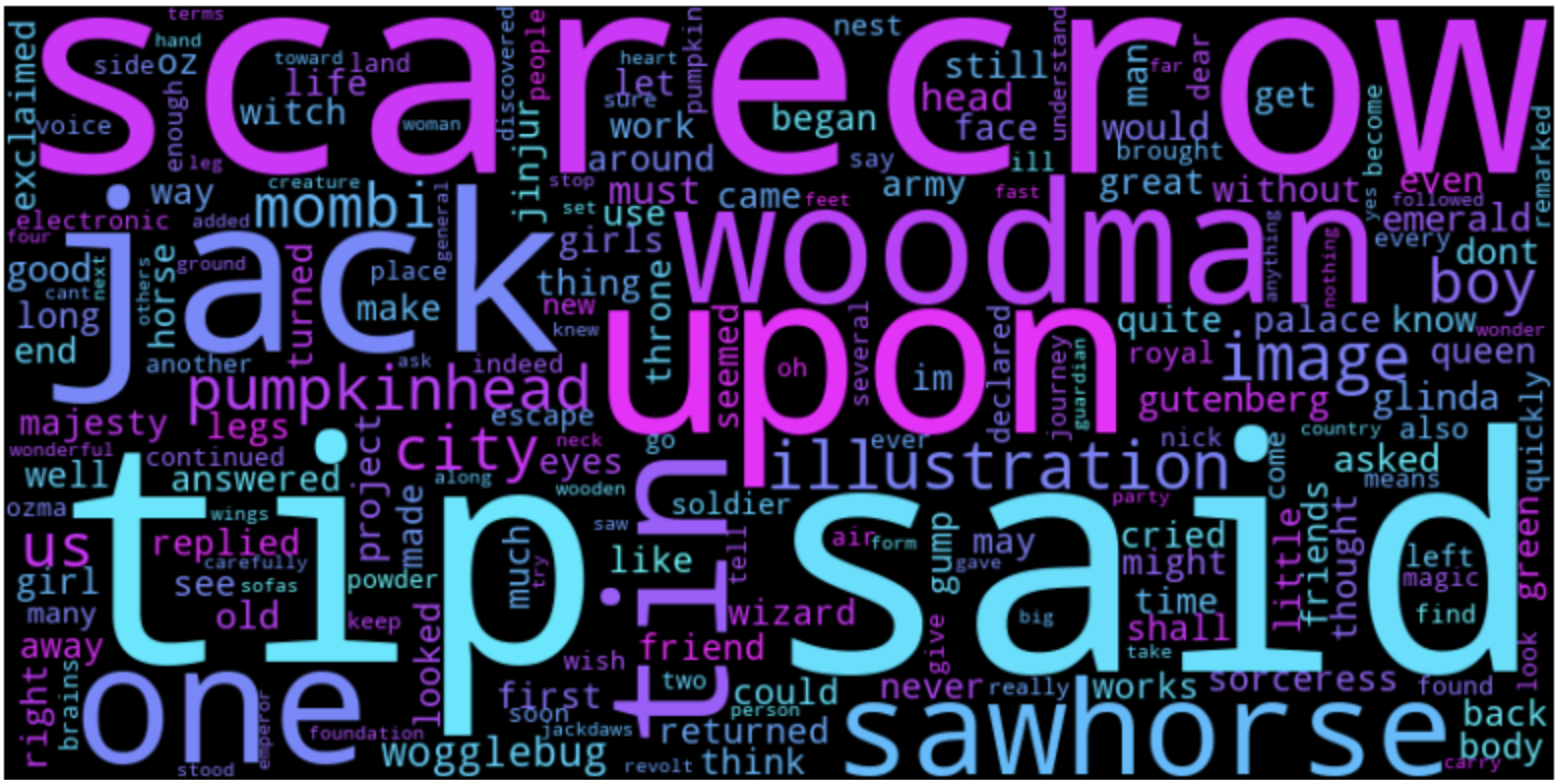
\includegraphics[width=0.8\linewidth]{Libro 1 WordCloud.png}
    \caption{WordCloud Libro 1.}
    \label{fig:Libro 1 WordCloud}
	\end{figure}

	\FloatBarrier

Al obtener el top 20 de palabras con mayor frecuencia obtenemos la siguiente lista: \texttt{said, tip, scarecrow, upon, jack, woodman, tin, one, sawhorse, illustration, image, pumpkinhead, city, mombi, boy, us, wogglebug, head, must} y \texttt{old}. Lo anterior se puede observar en la figura \ref{fig:Libro 1 Top 10}.  

	\begin{figure}[h]
    \centering
    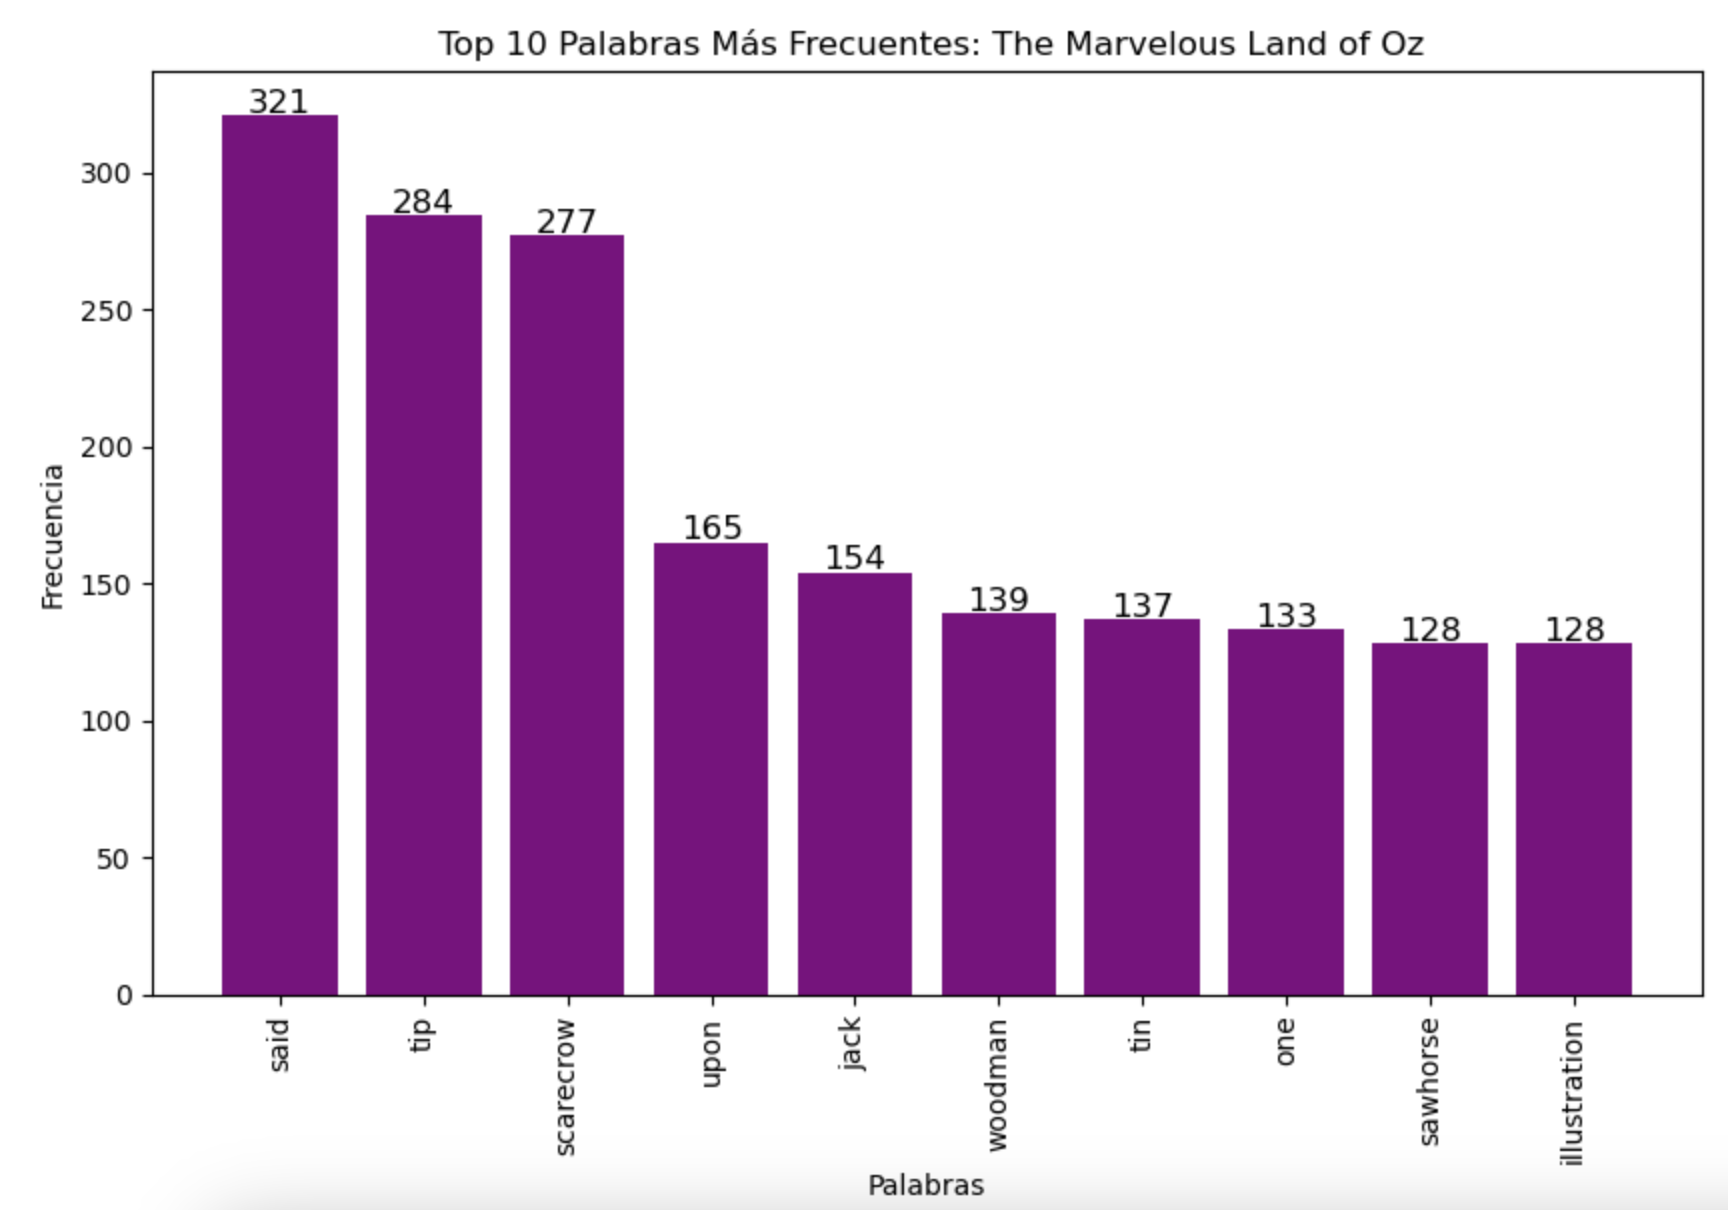
\includegraphics[width=0.9\linewidth]{Libro 1 Top 10 palabras más frecuentes.png}
    \caption{Top 10 Libro 1.}
    \label{fig:Libro 1 Top 10}
	\end{figure}

	\FloatBarrier


\subsubsection{Libro 2. Dorothy and the Wizard in Oz}

Para el segundo libro se obtuvo la siguiente nube de palabras:

	\begin{figure}[h]
    \centering
    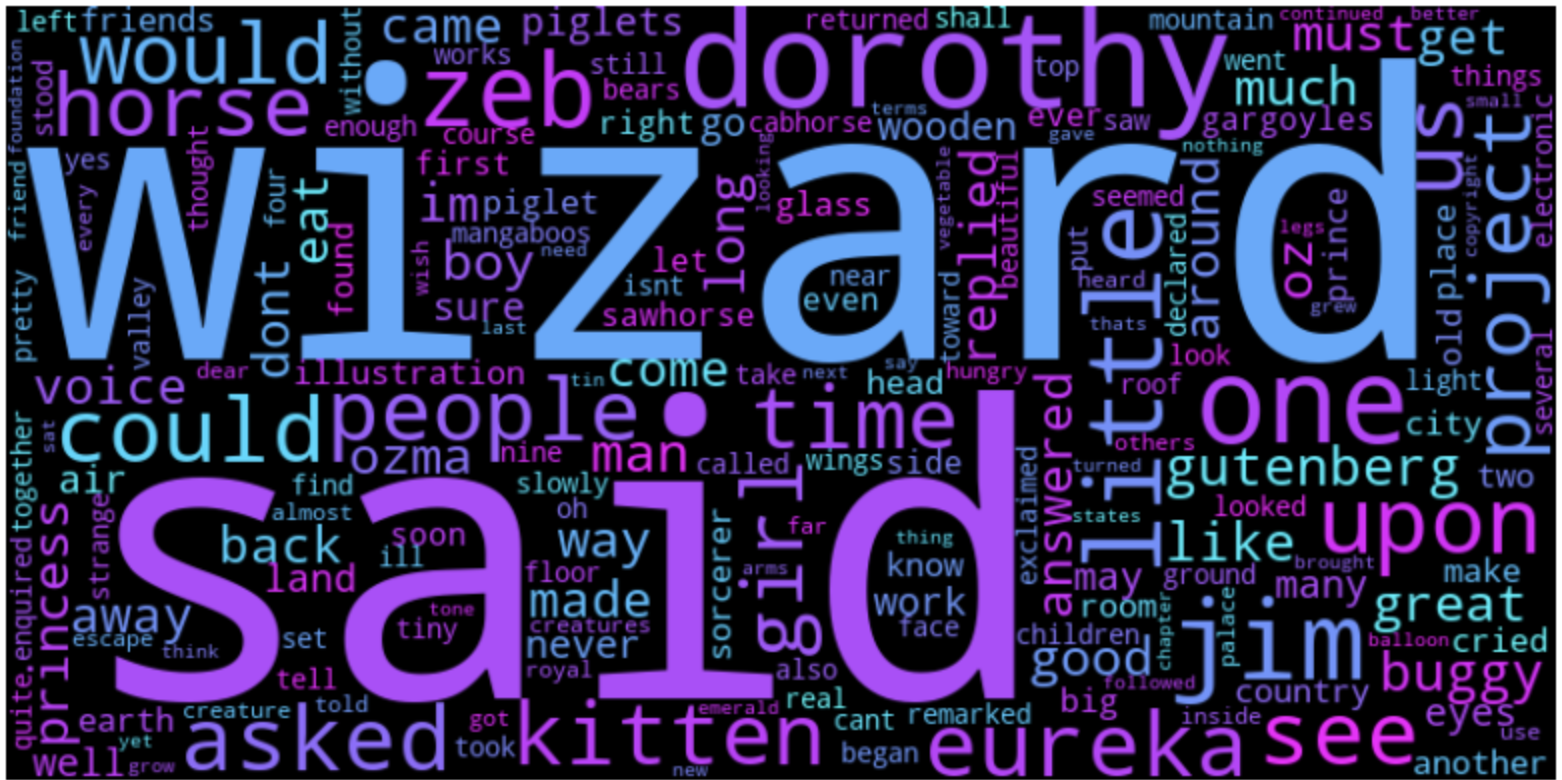
\includegraphics[width=0.8\linewidth]{Libro 2 WordCloud.png}
    \caption{WordCloud Libro 2.}
    \label{fig:Libro 2 WordCloud}
	\end{figure}

	\FloatBarrier

Al obtener el top 20 de palabras con mayor frecuencia obtenemos la siguiente lista: \texttt{said, wizard, dorothy, one, jim, little, zeb, upon, could, asked, eureka, see, people, kitten, horse, time, would, us, girl} y \texttt{project}. Lo anterior se puede observar en la figura \ref{fig:Libro 2 Top 10}.  

	\begin{figure}[h]
    \centering
    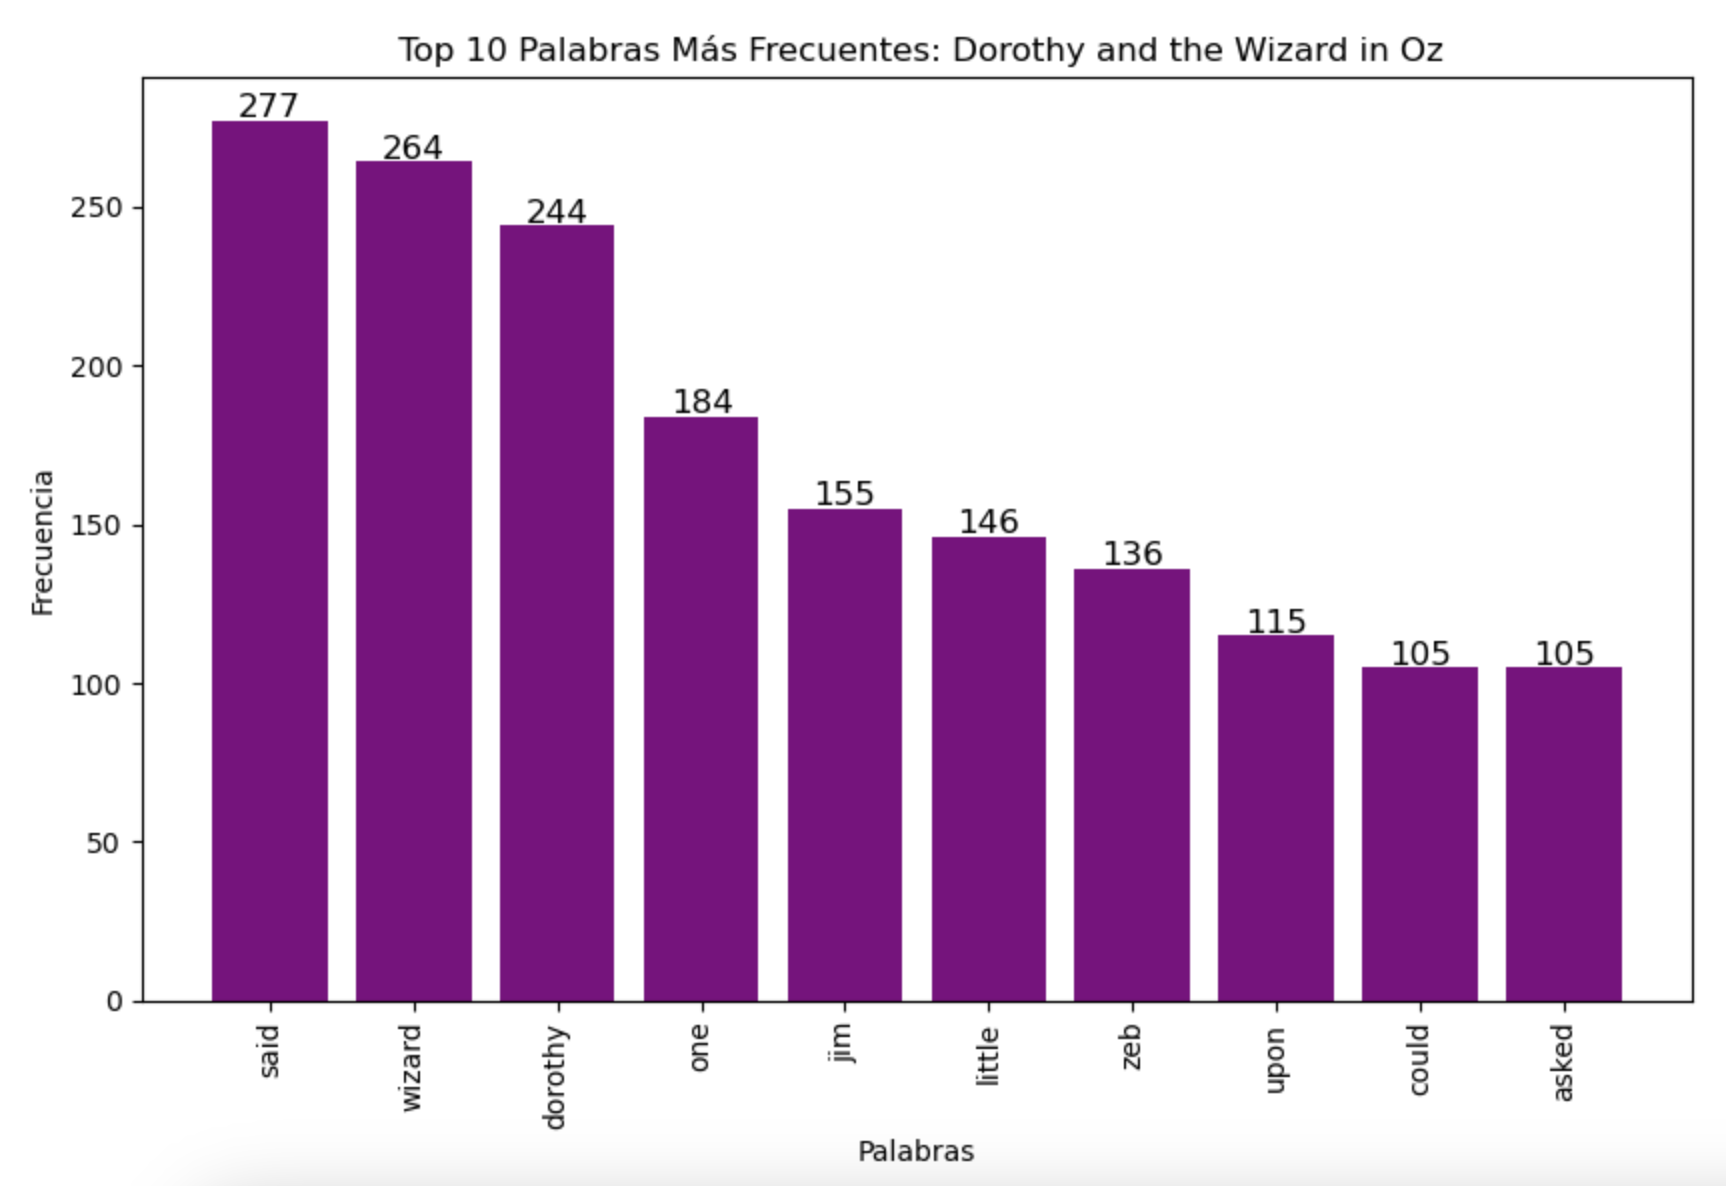
\includegraphics[width=0.9\linewidth]{Libro 2 Top 10 palabras más frecuentes.png}
    \caption{Top 10 Libro 2.}
    \label{fig:Libro 2 Top 10}
	\end{figure}

	\FloatBarrier

\newpage 

\subsubsection{Libro 3. The Magic of Oz}

Para el tercer libro se obtuvo la siguiente nube de palabras:

	\begin{figure}[h]
    \centering
    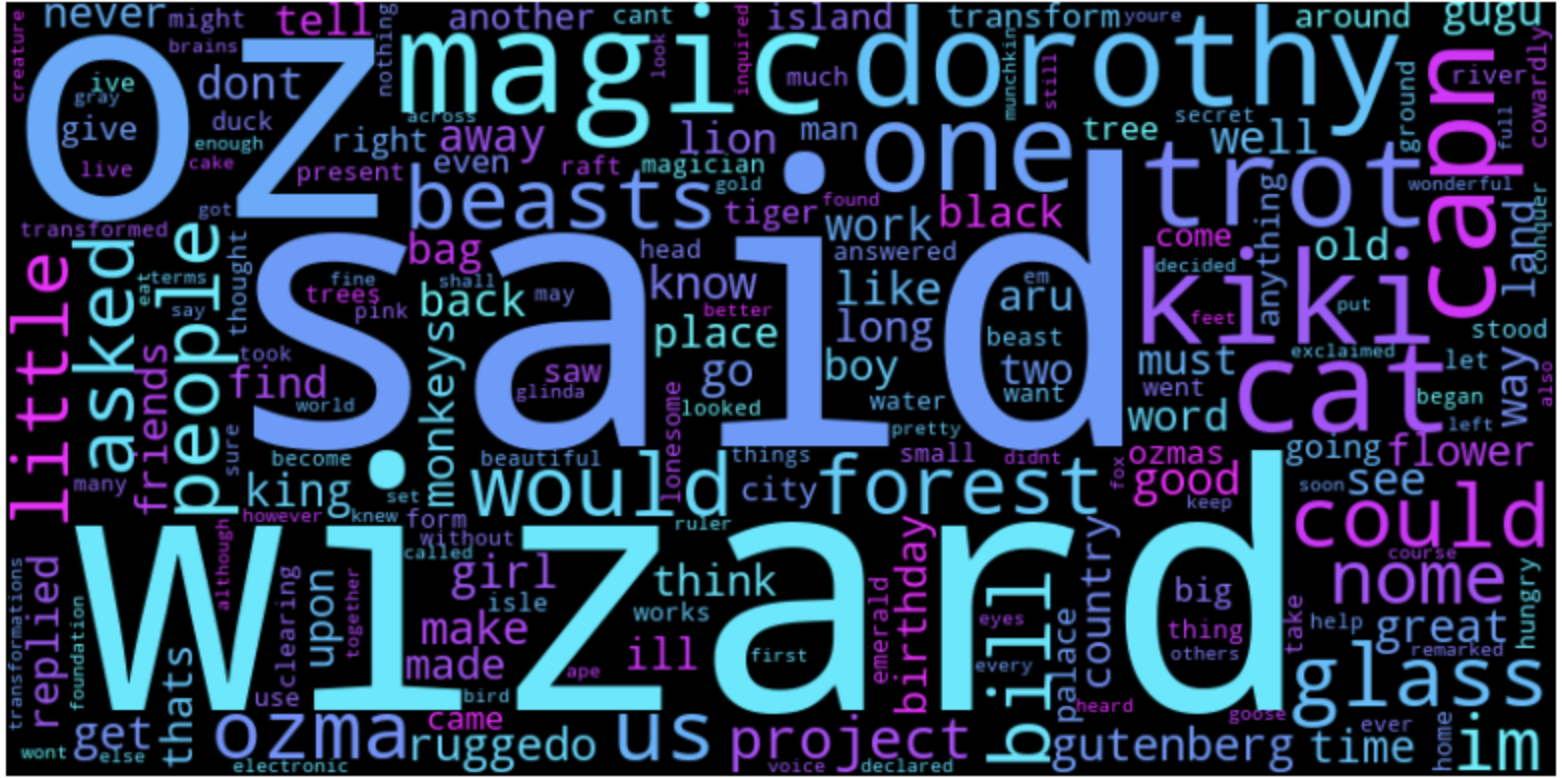
\includegraphics[width=0.8\linewidth]{Libro 3 WordCloud.png}
    \caption{WordCloud Libro 3.}
    \label{fig:Libro 3 WordCloud}
	\end{figure}

	\FloatBarrier

Al obtener el top 20 de palabras con mayor frecuencia obtenemos la siguiente lista: \texttt{said, wizard, oz, magic, dorothy, kiki, cat, trot, one, capn, glass, could, would, beasts, us, bill, people, ozma, forest} y \texttt{asked}. Lo anterior se puede observar en la figura \ref{fig:Libro 3 Top 10}.  

	\begin{figure}[h]
    \centering
    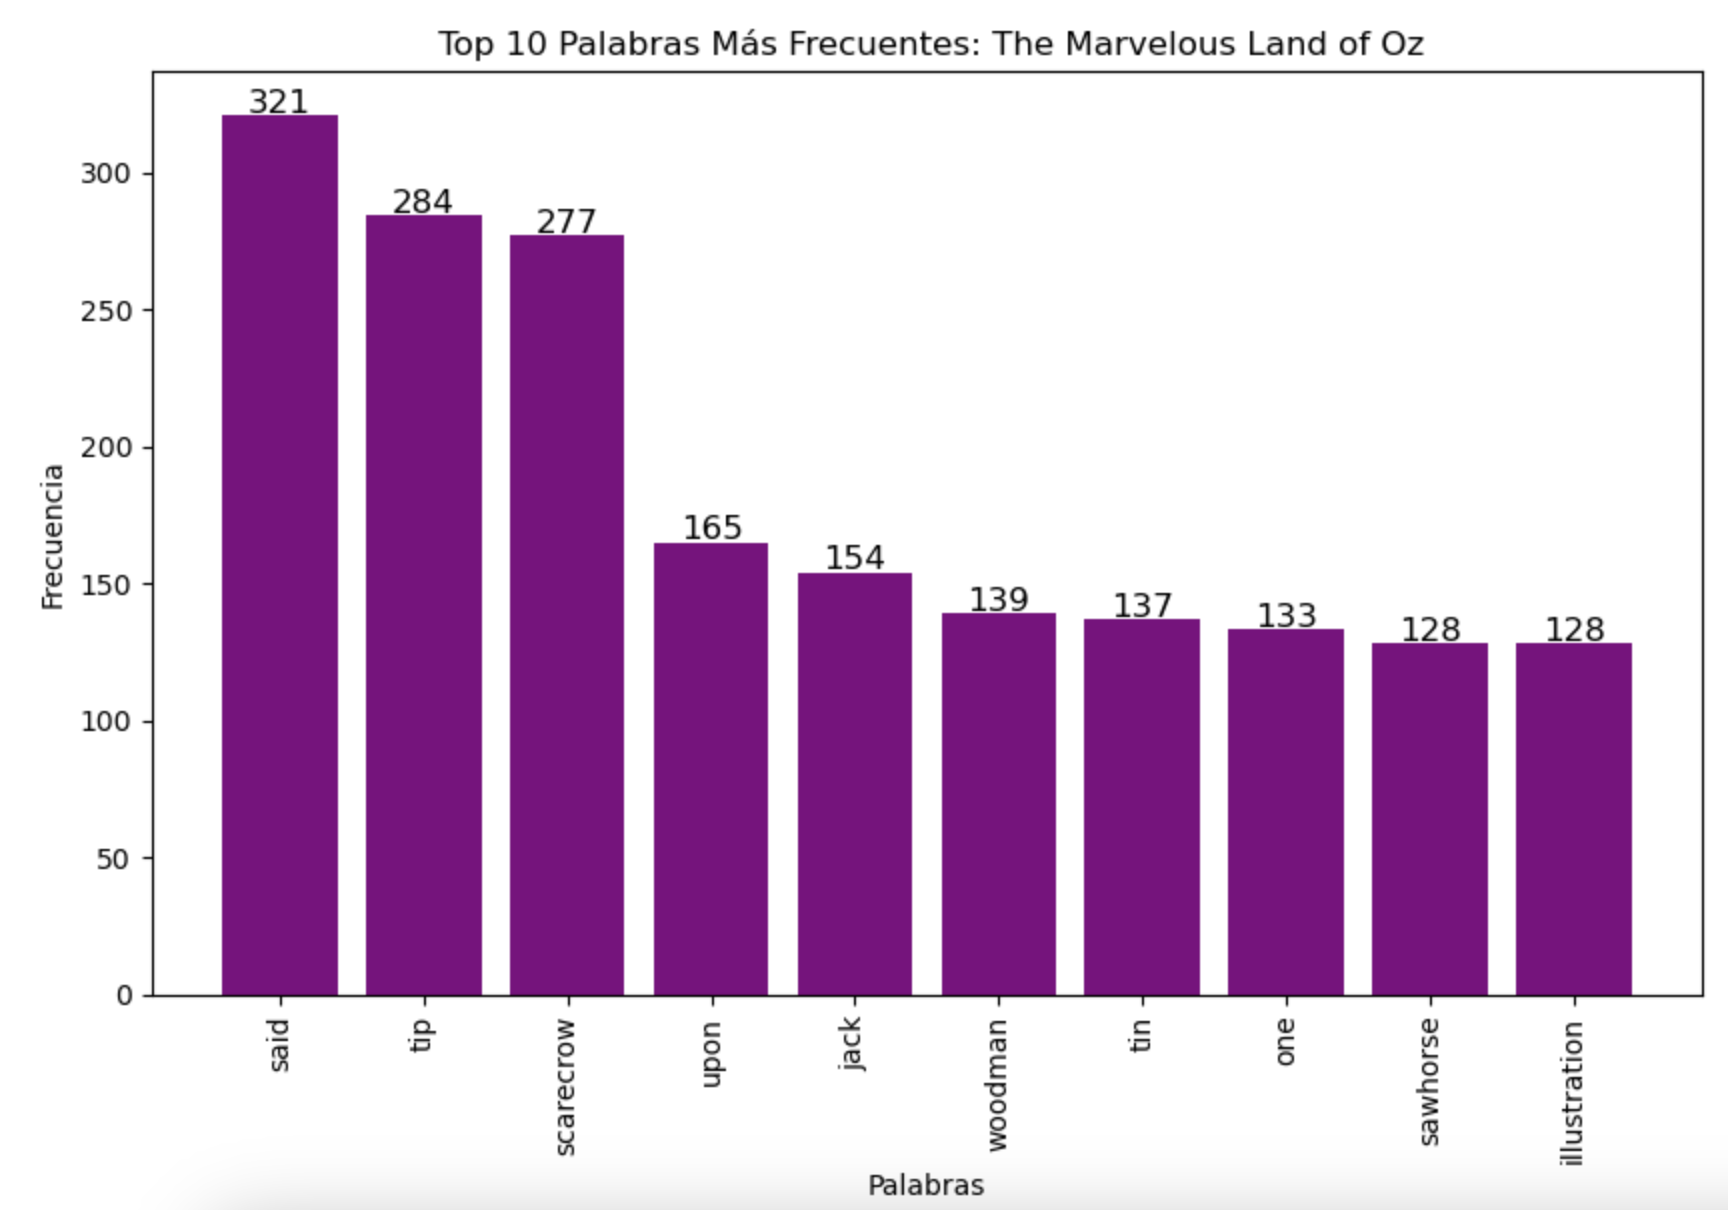
\includegraphics[width=0.9\linewidth]{Libro 1 Top 10 palabras más frecuentes.png}
    \caption{Top 10 Libro 3.}
    \label{fig:Libro 3 Top 10}
	\end{figure}

	\FloatBarrier


\subsection{Comparación entre Fuentes}

El análisis cruzado reveló diferencias en el enfoque de cada libro, a pesar de ser del mismo autor. Mientras que algunos textos priorizan la descripción, otros favorecen la acción directa y el diálogo. Las métricas de bigramas y trigrams evidencian estas variaciones estilísticas.


	\begin{figure}[h]
    \centering
    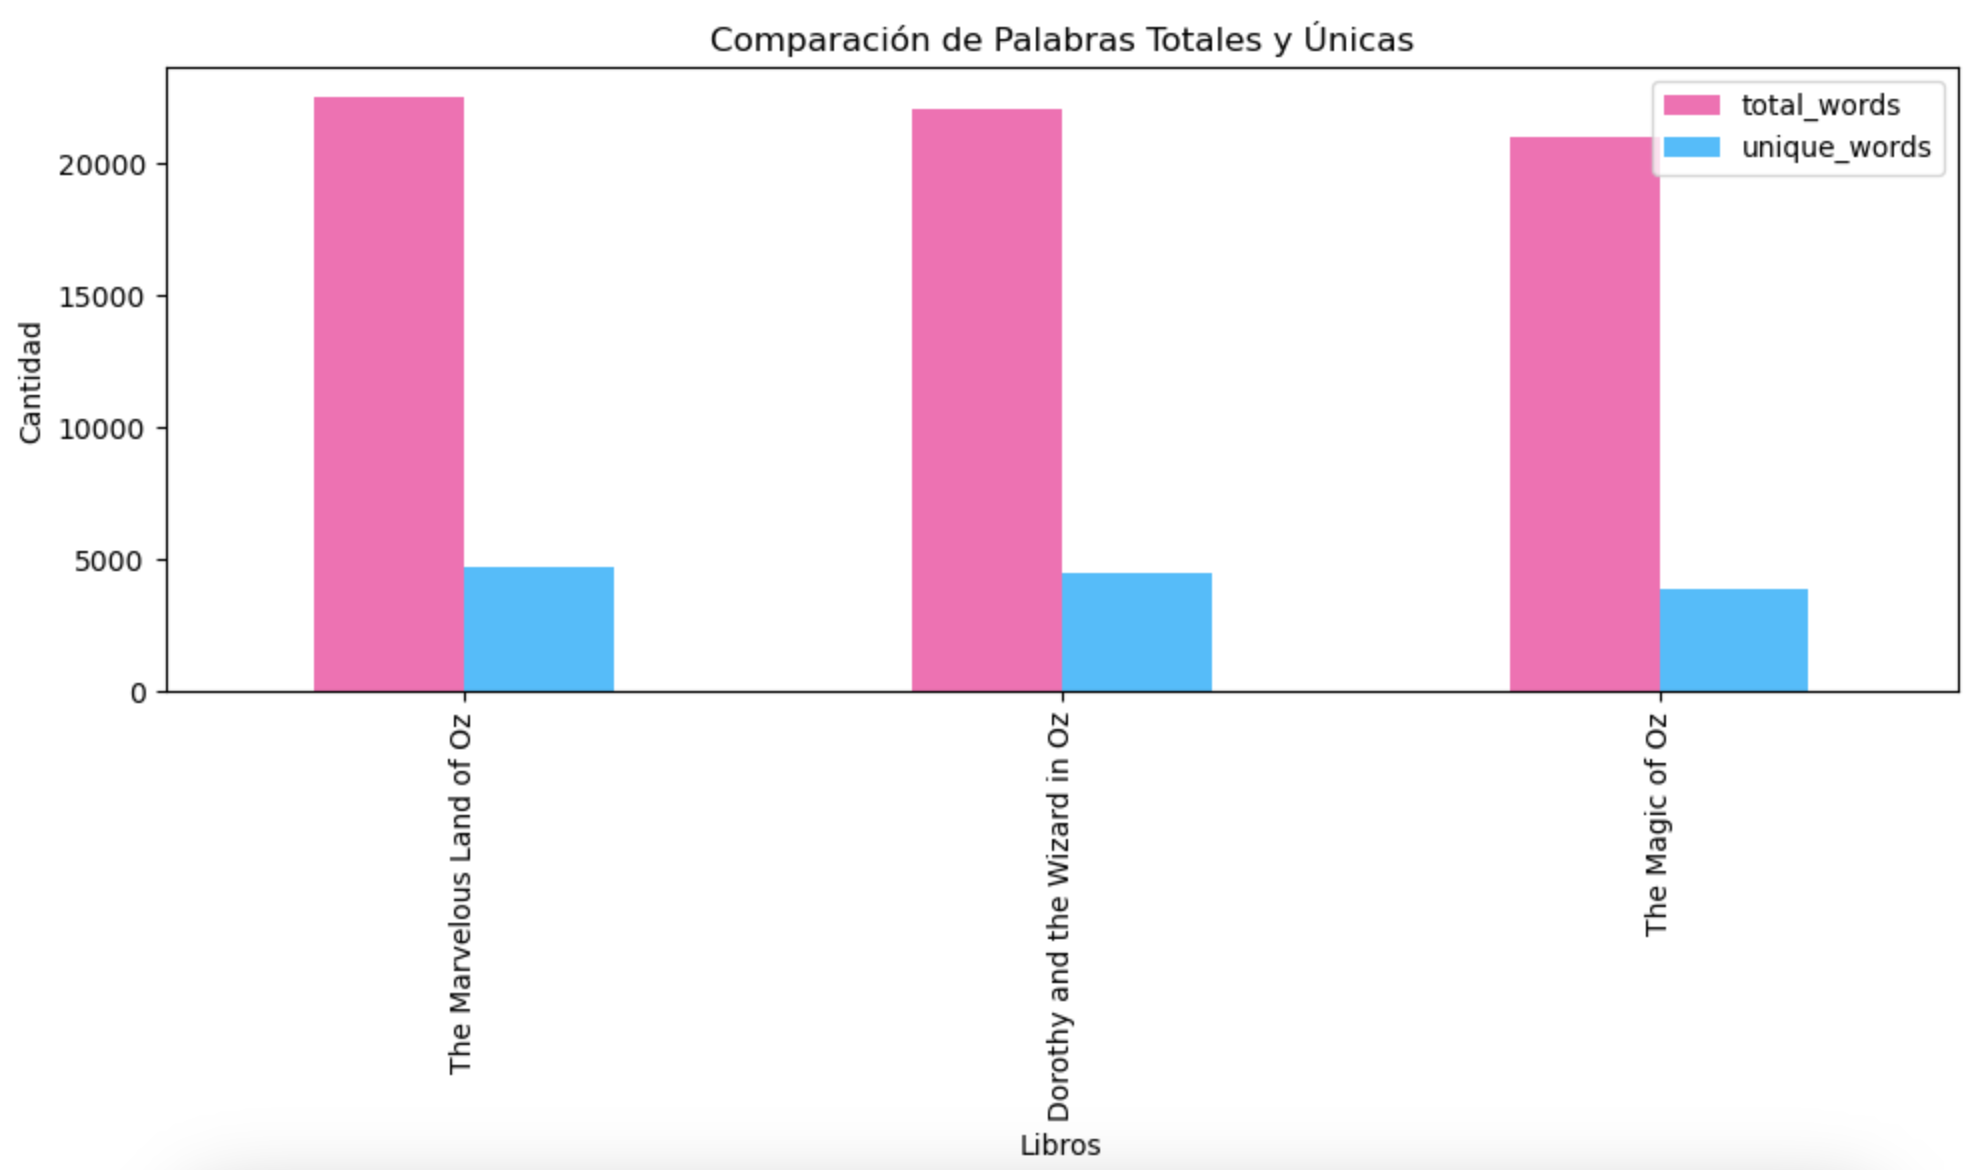
\includegraphics[width=0.9\linewidth]{Comparación de palabras totales y únicas.png}
    \caption{Comparación entre los 3 libros.}
    \label{fig:Comparación}
	\end{figure}

	\FloatBarrier

Adicional a la comparación que se muestra en la \ref{fig:Comparación} se obtuvo una lista con las palabras del top 20 que tengan en común los libros:

\begin{itemize}

\item Palabras comunes en los libros 1 y 2: \texttt{said, one, us, upon}.

\item Palabras comunes en los libros 2 y 3: \texttt{one, people, us, said, would, dorothy, wizard, could, asked}.

\item Palabras comunes en los libros 1 y 3: \texttt{said, one, us}.

\item Palabras comunes en los 3 libros:\texttt{ said, one, us}.

\end{itemize}



\section{Conclusiones}

Este estudio demuestra la eficacia de las herramientas computacionales en el análisis textual. Las principales conclusiones incluyen:

\begin{itemize}

    \item \textbf{Relevancia de las herramientas computacionales: }Las técnicas empleadas, como la tokenización y la eliminación de palabras vacías, facilitaron la extracción de patrones lingüísticos clave, evidenciando diferencias estilísticas significativas entre las obras analizadas. Esto refuerza la utilidad de enfoques automatizados en el estudio de grandes volúmenes de texto.

    \item \textbf{Visualizaciones intuitivas:} El uso de nubes de palabras y gráficos de frecuencia resultó fundamental para comunicar hallazgos complejos de manera accesible y comprensible. Estas representaciones gráficas no solo destacan los términos más relevantes, sino que también permiten detectar rápidamente las características distintivas de cada obra.

    \item \textbf{Diferencias estilísticas entre obras:} A pesar de compartir el mismo autor, las obras presentan variaciones notables en sus estructuras narrativas. Mientras que algunas priorizan descripciones detalladas, otras se centran más en el diálogo y la acción, lo que fue evidenciado a través de análisis de bigramas y trigramas.
    
\end{itemize}

En futuras investigaciones, se podrían incorporar técnicas de análisis de sentimientos y modelos de aprendizaje automático para profundizar en el entendimiento del contenido textual.

\end{document}
